\documentclass{article}

\usepackage[margin=0.5in,bottom=1in,footnotesep=1in]{geometry}

\usepackage{amsmath}


\usepackage{multicol}
\setlength{\columnsep}{1cm}
\usepackage[]{algorithm2e}

\usepackage{lipsum}% for dummy text
\usepackage[varg]{txfonts}
\usepackage{graphicx}
\usepackage{subcaption}
\usepackage{multirow}

\usepackage[font=small,labelfont={sf,bf}]{caption}

\usepackage{color}

\usepackage[export]{adjustbox}

\usepackage{titlesec}
\titleformat{\section}{\fontfamily{phv}\fontsize{12}{15}\bfseries}{\thesection}{1em}{}
\titleformat{\subsection}{\fontfamily{phv}\fontsize{10}{15}\itshape}{\thesubsection}{1em}{}
\titleformat{\subsubsection}{\fontfamily{phv}\fontsize{9}{15}\bfseries}{\thesubsubsection}{1em}{}


\title{\textbf{FYS4150 Project 4: \\The Ising model in two dimensions}}
\author{Marie Foss (\# 56), Maria Hammerstr{{\o}}m (\# 59)}
\date{}

\begin{document}

\maketitle

\begin{abstract}
	\noindent We study the Ising model in two dimensions for different lattice sizes $L$ and estimates the critical temperature $T_{\mathrm{C}}$ of the system as it experiences a magnetic phase transition using Monte Carlo simulations. FINDINGS, etc.
	% \lipsum[1]
	\vspace*{2ex}
	
	\noindent \textbf{Github:} \textit{https://github.com/mariahammerstrom/Project4}
	\vspace*{2ex}
\end{abstract}



\begin{multicols}{2}

\section{Introduction}

In this project we study the Ising model in two dimensions without an external magnetic field. The Ising model is used to study phase transitions at finite temperature for magnetic systems. The model was invented in 1920\footnote{Lenz, W. (1920). "Beitr�ge zum Verst�ndnis der magnetischen Eigenschaften in festen K�rpern". \textit{Physikalische Zeitschrift} 21: 613-615.} and the analytical solution to the two-dimensional case was found in 1944\footnote{Onsager, Lars (1944). "Crystal statistics. I. A two-dimensional model with an order-disorder transition". \textit{Physical Review}, Series II 65 (3-4): 117-149.}.




\subsection{Theory}\label{subsec:theory}
In the two-dimensional Ising model, the simplest form of the \textbf{energy} for a specific microstate $i$ is expressed as

\begin{equation}\label{eq:energy}
	E_i = -J \sum_{\langle kl\rangle}^{N}s_k s_l,
\end{equation}
with  $s_k=\pm 1$ where $+ 1$ denotes spin up and $ - 1$ denotes spin down, $N$ is the total number of spins and $J$ is a coupling constant expressing the strength of the interaction between neighbouring spins. The symbol $\langle kl\rangle$ indicates that the sum is over nearest neighbours only. We assume ferromagnetic ordering, meaning $J> 0$ and will make use of periodic boundary conditions.

The probability of finding the system in a given microstate $i$ is expressed by the \textbf{Boltzmann probability distribution}

\begin{equation}
	P_i (\beta) = \frac{e^{-\beta E_i}}{Z},
\end{equation}
where $\beta = 1/kT$ with $k$ the Boltzmann constant and $T$ the temperature, and with $Z$ as the \textbf{partition function} for the canonical ensemble defined as

\begin{equation}\label{eq:partition_func}
	Z = \sum_{i = 1}^{\infty} e^{-\beta E_i},
\end{equation}
summing over all micro states $i$. 

The \textbf{magnetic moment} of a given microstate is

\begin{equation}\label{eq:magnetization}
	{\cal M}_i = \sum_j s_j.
\end{equation} 
Some quantities of interest are the \textbf{expectation values} for the energy $\langle E\rangle$ and magnetic moment $\langle {\cal M}\rangle$:

\begin{equation}
\begin{aligned}
	\langle E \rangle &= \frac{1}{Z} \sum_i E_i e^{- \beta E_i} = kT^2 \frac{\partial \textrm{ ln } Z}{\partial T} = - \frac{\partial \textrm{ ln } Z}{\partial \beta} \\
	\langle {\cal M}\rangle &= \frac{1}{Z} \sum_i {\cal M}_i e^{- \beta E_i},
\end{aligned}
\end{equation}
as well as the \textbf{variances} for the energy $\sigma_E^2$ and for the magnetic moment $\sigma_M^2$, describing how the calculated values of $E$ and $M$ deviates from the expectation values:

\begin{equation}\label{eq:expect_values}
\begin{aligned}
	\sigma_E^2 &= \langle E^2\rangle - \langle E\rangle^2 \\
	\sigma_{\cal M}^2 &= \langle {\cal M}^2\rangle - \langle {\cal M}\rangle^2,
\end{aligned}
\end{equation}
These values can be used to calculate the \textbf{heat capacity} of a fixed volume given by

\begin{equation}
	C_V = \frac{\sigma_E^2}{kT^2} = \frac{\partial \langle E\rangle}{\partial T},
\end{equation}
and the \textbf{susceptibility}, which describes whether a material is attracted into or repelled out of a magnetic field, given by

\begin{equation}
	\chi = \frac{\sigma_{\cal M}^2}{kT} = \frac{\langle {\cal M}^2\rangle - \langle {\cal M}\rangle^2}{kT}.
\end{equation}
We want to compute these quantities after the system has \textbf{thermalized}, which is when the system has reached its most likely state. This will depend on the temperature $T$.

The model we are considering here undergoes a \textbf{phase transition}. Below a critical temperature $T_{\mathrm{C}}$ there is spontaneous magnetization $\langle {\cal M}\rangle \neq 0$ (magnetic phase), while above this temperature the average magnetization is zero (paramagnetic phase). Near $T_{\mathrm{C}}$ we can characterize the behaviour of many physical quantities by a power law behaviour.

An important quantity is the \textbf{correlation length}, which is expected to be of the order of the lattice spacing for $T \gg T_{\mathrm{C}}$. Because the spins become more and more correlated as $T$ approaches $T_{\mathrm{C}}$, the correlation length increases as we get closer to the critical temperature. The divergent behaviour of $\xi$ near $T_{\mathrm{C}}$ is

\begin{equation}\label{eq:xi}
	\xi(T) \sim \left|T_{\mathrm{C}} - T\right|^{-\nu}.
\end{equation}
A second-order phase transition is characterized by a correlation length which spans the whole system. Since we are always limited to a finite lattice, $\xi$ will be proportional with the size of the lattice. Through so-called finite size scaling relations it is possible to relate the behaviour at finite lattices with the results for an infinitely large lattice. The critical temperature then scales as

\begin{equation}\label{eq:T_C}
	T_{\mathrm{C}}(L) - T_{\mathrm{C}}(L=\infty) = aL^{-1/\nu},
\end{equation}
with $a$ a constant and $\nu$ defined in Eq.~(\ref{eq:xi}). In this project we will use $\nu = 1$.




\subsection{Analytical solution}\label{subsec:analytical}
First we will assume that we only have two spins in each dimension, that is $L = 2$, where $L$ is the width of the lattice. The situation looks like this:

\begin{align*}
	\uparrow_{(1)} \quad &\uparrow_{(2)}   \\
	\uparrow_{(3)} \quad &\uparrow_{(4)}\,,   
\end{align*}
where an upward arrow denotes spin up and the numbers are just a way to identify the different spins. We will make use of \textbf{periodic boundary conditions}, which means that the neighbour to the right of a given spin $s_N$ takes the value of $s_1$. Similarly, the neighbour to the left of $s_1$ takes the value of $s_N$. This way of treating the boundaries are often used when approximating an infinite system that has a repeating structure. In our case, this means that we will treat our system as though it looked like this (where the original system is highlighted in magenta):

\begin{align*}
	\textcolor{black}{\uparrow_{(4)}} \quad \textcolor{black}{\uparrow_{(3)}} \quad \textcolor{black}{\uparrow_{(4)}} \quad &\textcolor{black}{\uparrow_{(3)}} \\
	\textcolor{black}{\uparrow_{(2)}} \quad \textcolor{magenta}{\uparrow_{(1)}} \quad \textcolor{magenta}{\uparrow_{(2)}} \quad &\textcolor{black}{\uparrow_{(1)}} \\
	\textcolor{black}{\uparrow_{(4)}} \quad \textcolor{magenta}{\uparrow_{(3)}} \quad \textcolor{magenta}{\uparrow_{(4)}} \quad &\textcolor{black}{\uparrow_{(3)}} \\
	\textcolor{black}{\uparrow_{(2)}} \quad \textcolor{black}{\uparrow_{(1)}} \quad \textcolor{black}{\uparrow_{(2)}} \quad &\textcolor{black}{\uparrow_{(1)}}\,.
\end{align*}
Closed form expression can be found for the partition function in Eq. (\ref{eq:partition_func}), and the corresponding expectation values for $E$, $|{\cal M}|$, the specific heat $C_V$ and the susceptibility $\chi$ as functions of $T$ using periodic boundary conditions. In the case $L = 2$ we can write Eq. (\ref{eq:energy}) for the different components, making use of the periodic boundary conditions, giving

\begin{align*}
	E_1 &= - J (s_1 s_2 + s_1 s_3) = - 2J, \\
	E_2 &= - J (s_1 s_2 + s_2 s_4) = - 2J, \\
	E_3 &= - J (s_1 s_3 + s_3 s_4) = - 2J, \\
	E_4 &= - J (s_3 s_4 + s_2 s_4) = - 2J. 
\end{align*}
Thus the total energy for the system is

\begin{equation*}
	E = E_1 + E_2 + E_3 + E_4 = - 8J.
\end{equation*}
If going through this exercise for different configurations of spin up and spin down, we find values for energies, degeneracies and magnetization for different configurations as shown in Table~\ref{table:quantities}, where magnetization is calculated from Eq. (\ref{eq:magnetization}).

\begin{table*}
\begin{center}
\begin{tabular}{ l r r r }\hline
	Number of spins up 			& Energy $E$	 			& Degeneracy $\Omega$		& Magnetization ${\cal M}$		\\ \hline
	4 						& $- 8J$ 					& 1						& 4		 \\
	3 						& 0						& 4						& 2		 \\
	2						& 0						& 4						& 0		\\
	2						& $8J$					& 2						& 0		\\
	1						& 0						& 4						& -2		\\
	0						& $-8J$					& 1						& -4		\\
	\hline
\end{tabular}
\caption{Energy and magnetization for the two-dimensional Ising model with $N = 2 \times 2$ spins with periodic boundary conditions.}\label{table:quantities}
\end{center}
\end{table*}

These calculations can be used to find the closed-form expressions, starting with the partition function, which can be expressed as

\begin{align}\label{eq:Z_analytic}
	Z(\beta) 	&= \sum_E \Omega(E) e^{- \beta E} = 2 e^{8J\beta} + 2 e^{- 8J \beta} + 12 \\
			&= 4 \textrm{ cosh}(8J \beta) + 12.
\end{align}
Then the expectation value for the energy can be written, using the expression in Eq. (\ref{eq:expect_values}), as

\begin{equation}\label{eq:E_avg_analytic}
	\langle E\rangle = - \frac{8J \textrm{ sinh}(8J \beta)}{\textrm{cosh}(8J\beta) + 3} \approx - 8J \textrm{ tanh} (8J\beta),
\end{equation}
where we have used that cosh$(8J\beta) \gg 3$ in the approximation. Using this approximation gives

\begin{equation}\label{eq:C_V_analytic}
	C_V(\beta) = k \textrm{ } \bigg( \frac{8J\beta}{\textrm{cosh }(8J\beta)} \bigg)^2.
\end{equation}
Similarly, using the values for magnetization in Table~\ref{table:quantities} and Eq. (\ref{eq:magnetization}), gives

\begin{align}\label{eq:M_avg_analytic}
	\langle|{\cal M}|\rangle 	&= \frac{1}{Z} \bigg( 4e^{8J\beta} + 4\cdot2 + 4\cdot|-2| + |-4|e^{8J\beta} \bigg) \\
					&= \frac{8}{Z}(e^{8J\beta} + 2), \\
\end{align}
and
\begin{align}
	\langle {\cal M}\rangle 	&= \frac{1}{Z} \bigg( 4e^{8J\beta} + 4\cdot2 - 4\cdot2 - 4e^{8J\beta} \bigg) = 0, \\
	%\langle M\rangle^2 	&= 0 \\
	\langle {\cal M}^2\rangle 	&= \frac{1}{Z} \bigg( 4^2 e^{8J\beta} + 4\cdot2^2 + 4\cdot(-2)^2 + (-4)^2e^{8J\beta}   \bigg) \\
			&= \frac{32}{Z} \bigg( e^{8J\beta} + 1  \bigg).
\end{align}
Thus
\begin{equation}\label{eq:chi_analytic}
	\chi(\beta) = \frac{\langle {\cal M}^2\rangle - \langle {\cal M}\rangle^2}{kT} = \frac{32\beta}{Z} [e^{8J\beta} + 1] - \frac{\beta}{Z^2}[8e^{8J\beta} + 4]^2.
\end{equation}









\section{Methods}

We wrote a code for the Ising model in two dimensions which computes the mean energy $E$, mean magnetization $|{\cal M}|$, the specific heat $C_V$ and the susceptibility $\chi$ as functions of  $T$ using periodic boundary conditions for a lattice of size $L$ in the $x$ and $y$ directions. The total number of configurations is given by $2^N$ with $N = L \times L$ the number of spins for a lattice of width $L$. 

\subsection{Algorithm}
We made use of the \textbf{Metropolis algorithm}:

\begin{enumerate}
	\item Generate a random configuration in the lattice to create an initial state with energy $E_b$ ($b$ = beginning state).
	\item Change the initial configuration by flipping one spin. Compute the energy of this state $E_t$ ($t$ = trial state).
	\item Calculate $\Delta E = E_t - E_b$.
	\item \textit{The Metropolis test:} If $\Delta E \leq 0$ the new configuration is accepted, meaning the energy is lowered and we are moving towards the energy minimum at a given temperature. If $\Delta E > 0$, calculate $w = e^{- \beta \Delta E}$. If $w < r$ where $r$ is a random number between 0 and 1, accept the new configuration. Keep the old configuration otherwise.
	\item Compute the new energy $E' = E_t + \Delta E$. Calculate various expectation values using this energy.
	\item Repeat steps $2-5$ for the chosen number of Monte Carlo (MC) cycles, meaning the number of times we should sweep through the lattice.
	\item Compute the various expectation values by dividing by the total number of cycles (and possibly the number of spins).
\end{enumerate}
During the computation we want to check how many MC cycles we need before the system has reached its most likely state. This is done by comparing the new value of $E$ with the previous value of $E$. If the difference is smaller than $5 \%$, we can say that the most likely state has been reached. In total we run 1 million MC cycles.


\subsection{Parallelization}
We have parallelized our code using the Open MPI library. 


\subsection{Calculating $T_{\mathrm{C}}$}
The critical temperature $T_{\mathrm{C}}$ is described by Eq. (\ref{eq:T_C}), where $T_{\mathrm{C}}(L)$ is calculated for different lattice sizes $L$ through our algorithm described above.  $T_{\mathrm{C}}(L = \infty)$ is described by the exact value of 2.269 (in units of $kT/J$). The equation has two unknowns, $T_{\mathrm{C}}(L = \infty)$ and the constant $a$. By using our calculations for two different lattice sizes to calculate $T_{\mathrm{C}}(L)$, we can solve Eq. (\ref{eq:T_C}) in the two cases and get an estimate for $a$ and thus the critical temperature $T_{\mathrm{C}}$. 



\section{Results \& comments}

\subsection{Checking the 2 $\times$ 2 case}

Computing the mean energy $E$, mean magnetization $|{\cal M}|$, the specific heat $C_V$ and the susceptibility $\chi$ numerically with periodic boundary conditions, using the expressions from Sec.~\ref{subsec:theory}, gives results which can be compared with the results of the analytical closed-form expressions given in Sec.~\ref{subsec:analytical} to check that our code is working properly. 

For temperature $T=1.0$ (in units of $kT/J$), this gives the following results for a $2 \times 2$ spin system where the initial state has all spins pointing upwards:

\begin{center}
\begin{tabular}{ l l l }\hline
	Quantity 								& Closed form	 				& Numerical		\\ \hline
	Mean energy $E$ 						& $-8.00$ 						& $-8$		 \\
	Mean magnetization $|{\cal M}|$ 			& 3.99						& 4		 \\
	Specific heat $C_V$						& $2.88 \times 10^{-5}$			& 0 		\\
	Susceptibility $\chi$						& $8.02 \times 10^{-3}$			& 0		\\
	\hline
\end{tabular}
\end{center}
The numerical results follow that of Table \ref{table:quantities}. The result from the closed form expressions are not as good as the numerical result. However, since we have done some approximations in order to derive these closed form expressions, some deviation is expected. The minimum number of MC cycles needed to achieve good agreement for the expectation value for energy is calculated to be 22-24 cycles, which will vary slightly for each run, according to our energy difference test described earlier.

\begin{figure*}[t]
\begin{center}
\begin{tabular}{ccc}
  	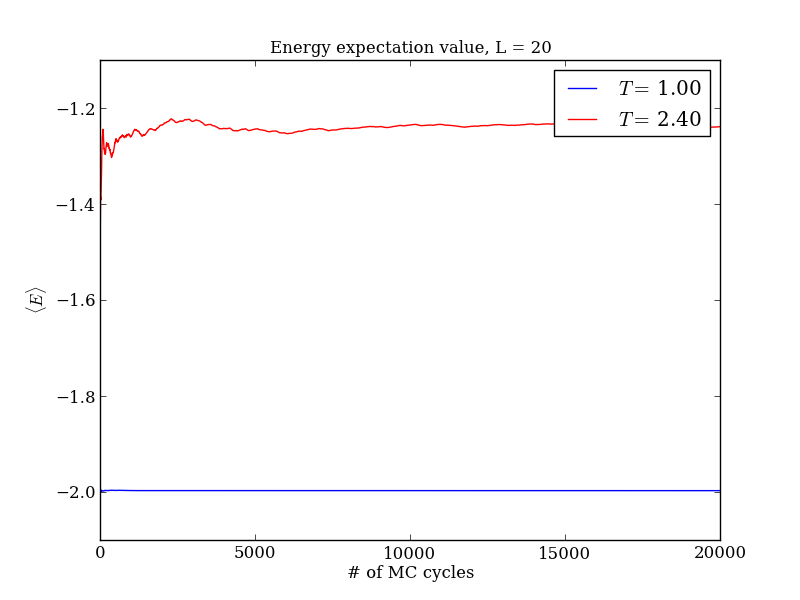
\includegraphics[width=85mm]{images/E_avg_MC_L20.png}
	& 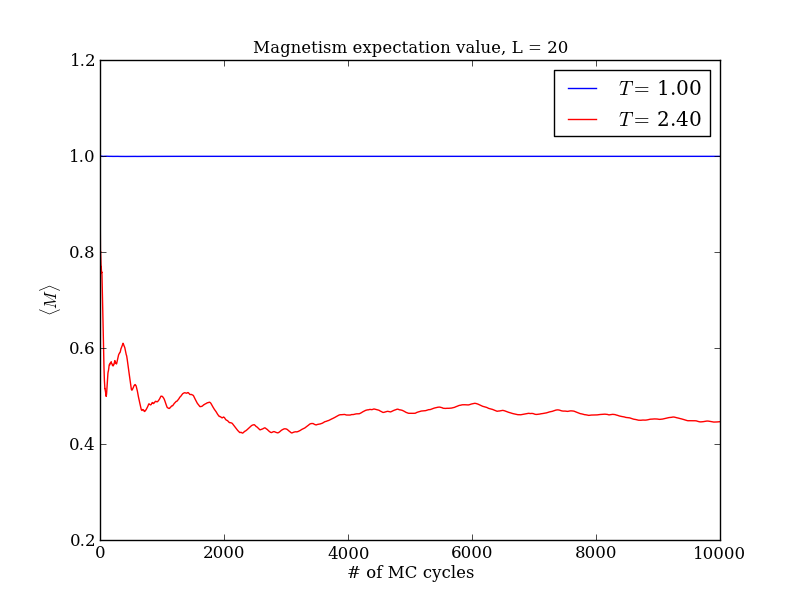
\includegraphics[width=85mm]{images/M_avg_MC_L20.png} \\
	(a) Energy					& (b) Magnetization  \\
	
	 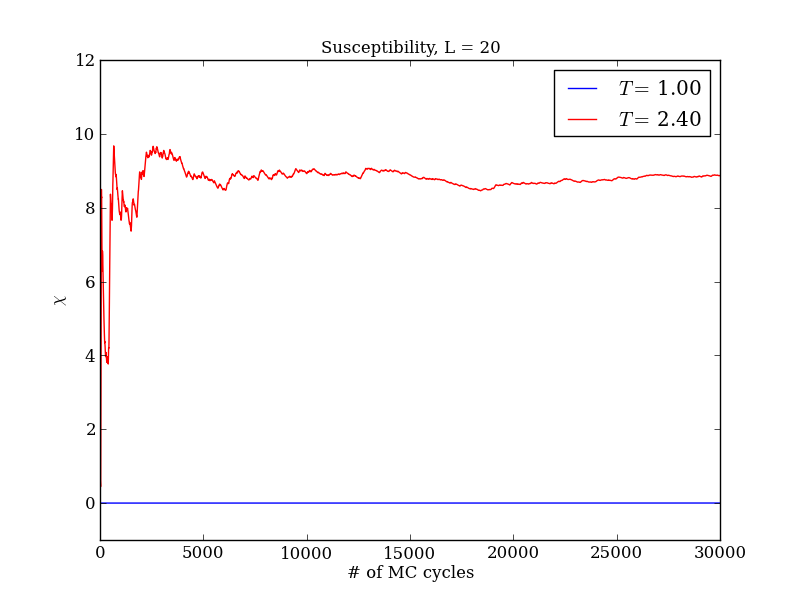
\includegraphics[width=85mm]{images/chi_MC_L20.png}
	& 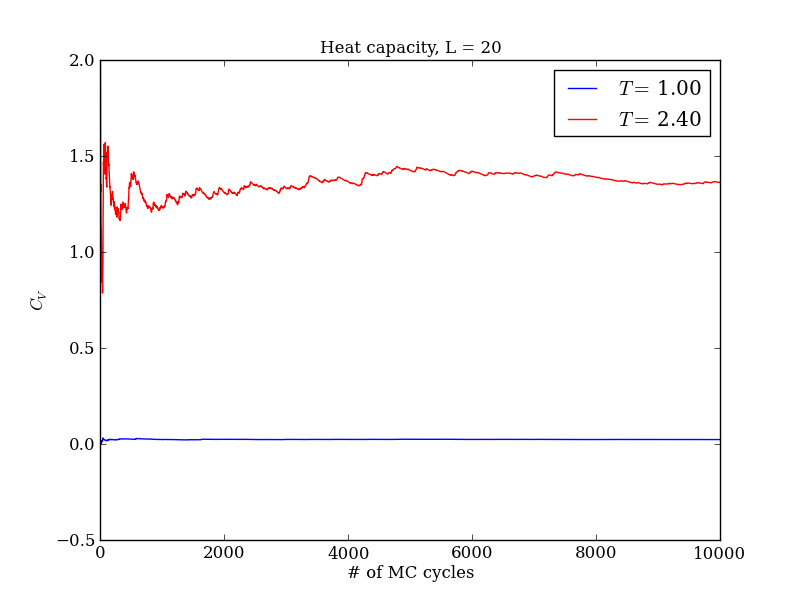
\includegraphics[width=85mm]{images/Cv_MC_L20.png} \\
	(c) Susceptibility					& (d) Heat capacity  \\[6pt]
\end{tabular}
\caption{Expectation values as a function of number of MC cycles with the hottest temperature in red (for an ordered initial spin state)).}\label{fig:L20_ex_values}
\end{center}
\end{figure*}


\subsection{The 20 $\times$ 20 case}
Next we looked at the case of $L = 20$ spins in the $x$ and $y$ directions. In this case we wanted to perform a study of the time (or number of MC cycles) we need before reaching an equilibrium situation and can start computing the various expectation values. A rough study is done by plotting the various expectation values as a function of number of MC cycles, for both $T = 1.0$ kT/J and $T = 2.4$ kT/J, as shown in Fig.~\ref{fig:L20_ex_values}a-d. 

For $T = 1.0$ kT/J, we see that the expectation values does not change considerably with the number of MC cycles, meaning the system reached the equilibrium state quickly. This is because we set all spin configurations to spin up for temperatures lower than $T=1.5$, meaning the system will be in its ground state of minimal energy right away. Here, as for the $L = 2$ case, the minimum number of MC cycles is around 22.

For $T = 2.4$ kT/J, on the other hand, the calculated values shows large variation for small numbers of MC cycles. The system reaches an equilibrium at a much later point. From studying the graphs in Fig.~\ref{fig:L20_ex_values}a-d this occurs after about 5000 MC cycles.  

Do these conclusions depend on whether we have an ordered (all spins pointing in one direction) or a random spin matrix as the starting configuration? Fig.~\ref{fig:random}a-b shows that for the low temperature of $T = 1.0$ kT/J the randomly oriented spin matrix will take longer to reach the most likely state, while the ordered spin matrix will hit the expectation value right away. This is different for a higher temperature. In the case of $T = 2.4$ kT/J both configurations deviate from the long-term expectation value in the beginning, then slowly oscillates towards a value close to the expectation value. 

\begin{figure*}[t]
\begin{center}
\begin{tabular}{c c c}
  	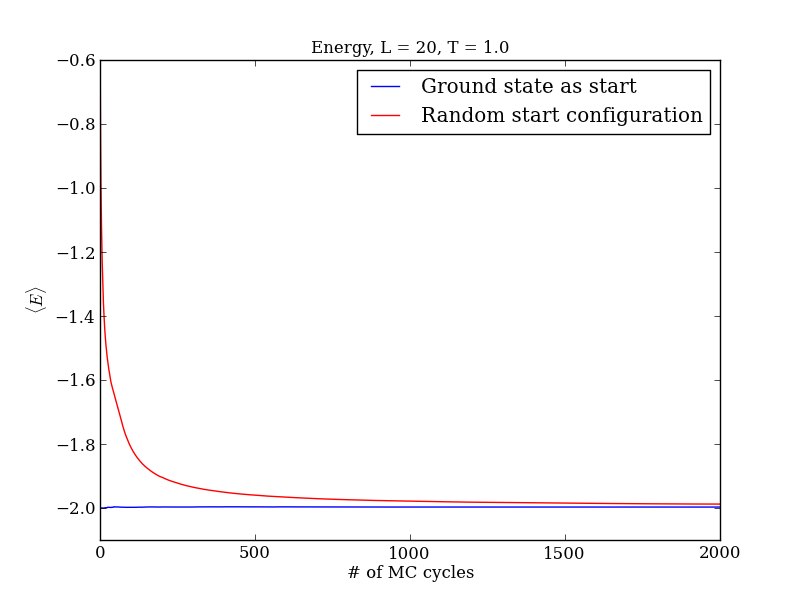
\includegraphics[width=85mm]{images/E_avg_MC_L20_random_T10.png}
	& 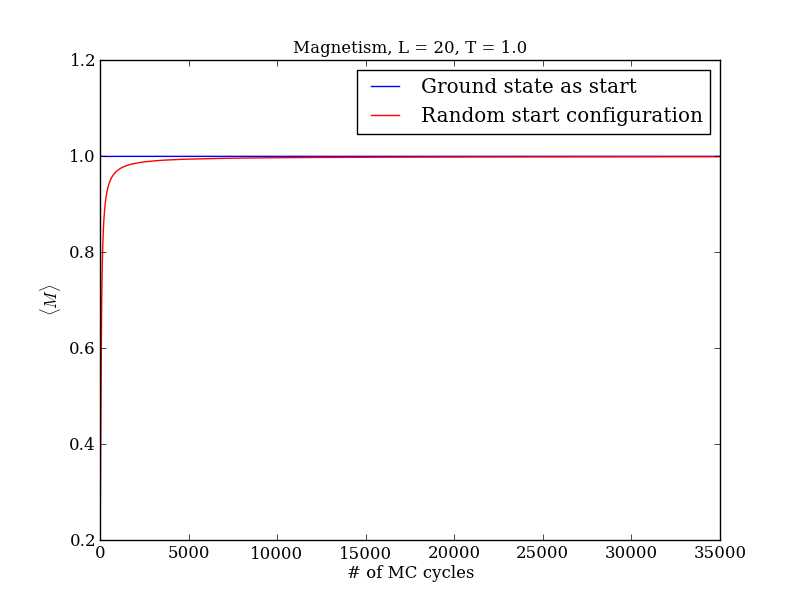
\includegraphics[width=85mm]{images/M_avg_MC_L20_random_T10.png} \\
	(a) Energy	, $T = 1.0$				& (b) Magnetization, $T = 1.0$  \\
	
	 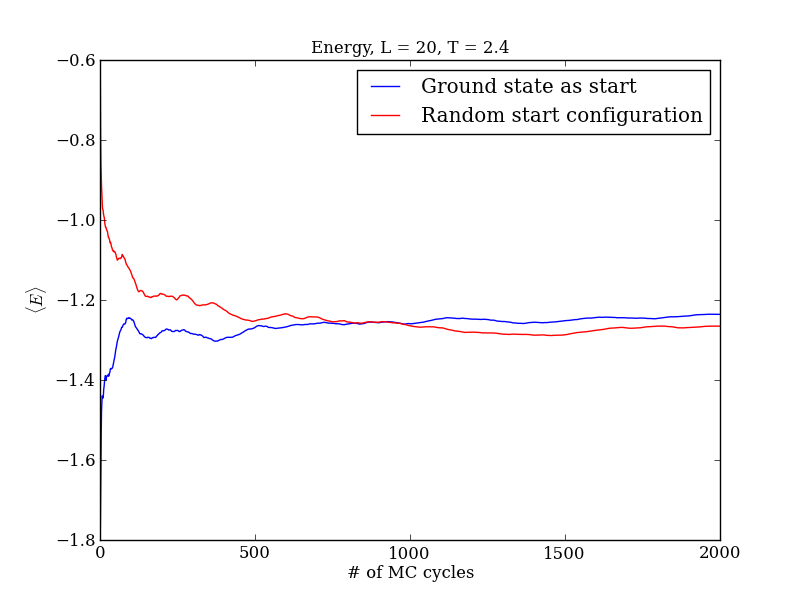
\includegraphics[width=85mm]{images/E_avg_MC_L20_random_T24.png}
	& 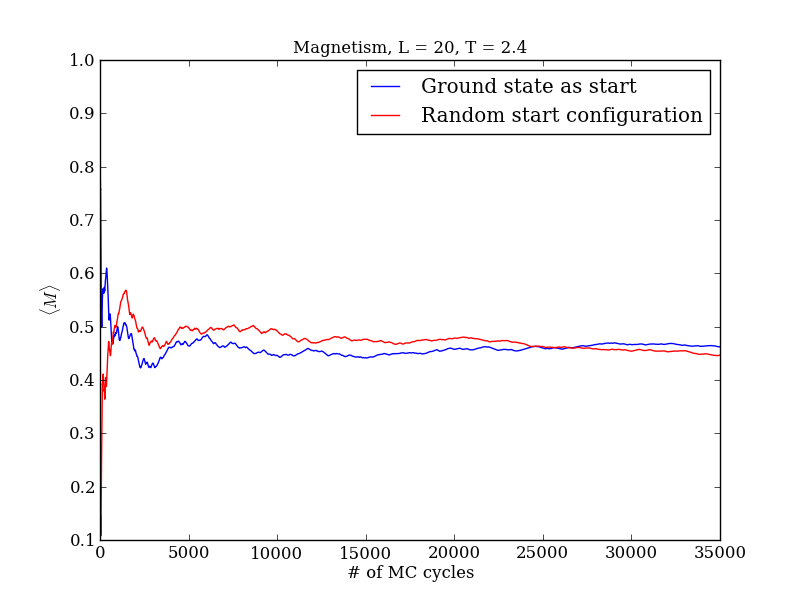
\includegraphics[width=85mm]{images/M_avg_MC_L20_random_T24.png} \\
	(c) Energy, $T = 2.4$				& (d) Magnetization, $T = 2.4$  \\[6pt]
\end{tabular}
\caption{Expectation values as a function of \# of Monte Carlo cycles with random and non-random initial spin matrix.}\label{fig:random}
\end{center}
\end{figure*}



\subsection{The number of accepted configurations}

The number of accepted configurations as a function of the total number of MC cycles is shown in Fig.~\ref{fig:L20_accepted_configs}a. The plot shows the number of accepted configurations divided by the total number of MC cycles. The number of accepted configurations scales approximately linearly with the total number of MC cycles. For $T=1.0$ kT/J there are no accepted configurations since no spin in the lattice is changed from up to down. 

For the case of $T = 2.4$ kT/J the number of accepted configurations increases rapidly in the beginning, then stabilizing, as the most likely state has been reached. 

\begin{figure*}[t]
\begin{center}
\begin{tabular}{ccc}
  	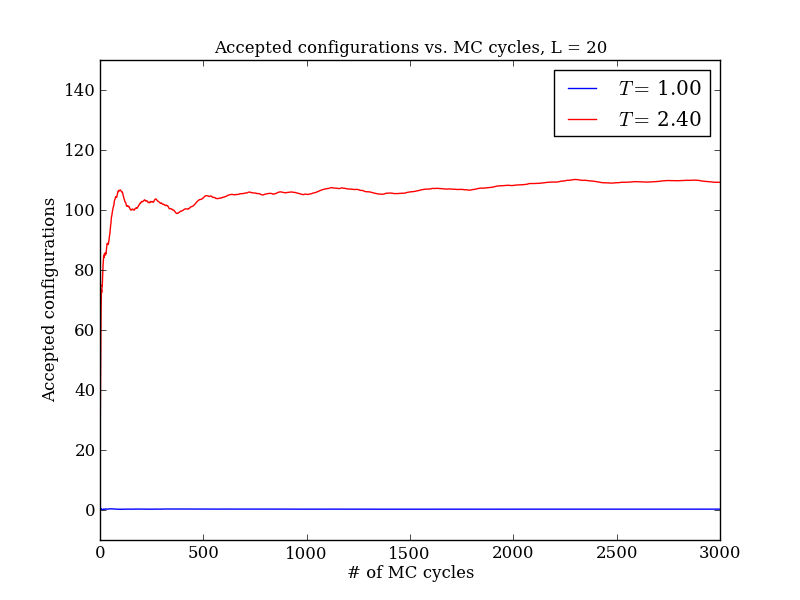
\includegraphics[width=85mm]{images/accepted_configs_MC_L20.png}
	& 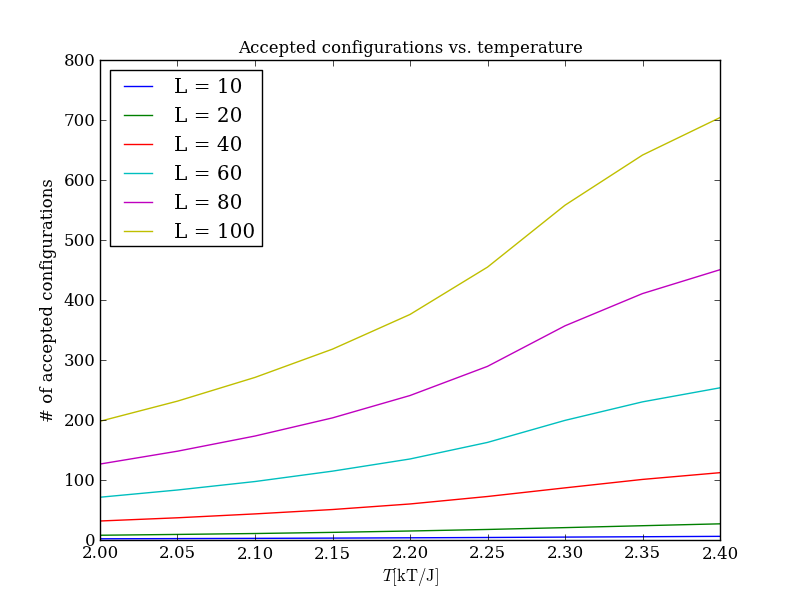
\includegraphics[width=85mm]{images/accepted_configs_temp.png} \\
	(a) As a function of \# of MC cycles.					& (b) As a function of temperature.  \\[6pt]
\end{tabular}
\caption{Number of accepted configurations.}\label{fig:L20_accepted_configs}
\end{center}
\end{figure*}
The total number of accepted configurations increases with higher temperature as shown in Fig.~\ref{fig:L20_accepted_configs}b. This is because of the test in the Metropolis algorithm saying that a configuration is accepted if $r < e^{-\Delta E/kT}$ where $r$ is a random number between 0 and 1. When the temperature is higher, $re^{-\Delta E/kT}$ will have a higher value, thus the probability of a spin flip is larger (as many more values of $r$ will fulfill the test), leading to more accepted configurations.

The figure also shows that this increase is greater with higher lattice size. This is natural as a larger lattice size means that we have a larger number of spins that can change direction, creating the possibility of many more accepted configurations. 



\subsection{The probability P(E)}

By simply counting the number of times a given energy appears in our computation, namely the expectation value for the energy, we can compute the probability $P(E)$ for getting that energy. We start the counting after the steady state situation has been reached, still looking at the $L = 20$ case. This result is compared with the computed variance in energy $\sigma_E^2$. 

For $T = 1.0$ kT/J we find that $P(E) = 0.87$ and $\sigma_E^2 = 0.02$, while for $T = 2.4$ kT/J we find that $P(E) = 0.03$ and $\sigma_E^2 = 8.28$ in the case of an ordered initial spin matrix (according to Fig.~\ref{fig:random} this result would not be different for a randomly oriented spin matrix because we are excluding the first number of Monte Carlo cycles where having a different initial configuration would make a difference). This means that where there is a small deviation in energy values, described by the variance, there will be a high probability of getting the specific value $E$. When the deviation is large as for $T=2.4$ kT/J, the probability of getting the value $E$ is small.


\subsection{Looking for phase transitions}

\begin{figure*}[b!]
\begin{center}
\begin{tabular}{ccc}
  	
\includegraphics[width=56mm,frame]{images/visualization_L80_T2_0_square.png}
	& 
\includegraphics[width=56mm,frame]{images/visualization_L80_T2_2_square.png}
	& 
\includegraphics[width=56mm,frame]{images/visualization_L80_T2_4_square.png} \\
	
	(a) $T = 2.0$					
	& (b) $T = 2.2$
	& (c) $T = 2.4$  \\[6pt]
\end{tabular}
\caption{Visualization of the spin matrix for a $80 \times 80$ lattice for different temperatures $T$. White = spin up, black = spin down.}\label{fig:visualization}
\end{center}
\end{figure*}

A phase transition in a magnetic system is defined as the transition between the ferromagnetic and paramagnetic phases of the system. The transition occurs at a critical point, often referred to as the Curie point, which is dependent on temperature. Beyond the critical point defined by a critical temperature $T_{\mathrm{C}}$ (see next subsection) the system will loose its magnetic properties and the magnetic spins will be randomly aligned in our case where there is no external magnetic field affecting the spin directions.

The spin matrix in the case of $L = 80$ for different temperatures is visualized in Fig.~\ref{fig:visualization}, where white squares represent upward spins and black squares represent downward spins. It shows clearly that the net magnetization $\langle {\cal M}\rangle$ is higher for low $T$ with most spins pointing in the same direction (in this case upwards), while the $\langle {\cal M}\rangle$ approaches zero at higher $T$ where the number of spins pointing upward and downward are about the same.

We see the same behaviour in Fig.~\ref{fig:ex_values_temp}b, which shows that for higher temperatures $\langle {\cal M}\rangle$ decreases more and more, with a particularly steep decrease around $T \approx 2.25$ and the value start to stabilize around $T \approx 2.35$ in the $L = 100$ case. Here $\langle {\cal M}\rangle$ approaches zero, meaning the net magnetization is expected to disappear more and more. This transition becomes steeper and steeper for increasing values of $L$.

These observations tells us that we might be witnessing a phase transition, going from an ordered, magnetic state to a random, nearly non-magnetized state.

Around the same temperature range the susceptibility and heat capacity also exhibits a clear change in behaviour. In the case of the susceptibility in Fig.~\ref{fig:ex_values_temp}c we see that the peak sharpens more and more for higher values of $L$, pointing us towards a critical temperature of $T_{\mathrm{C}} \approx 2.3$. Similar behaviour can be seen for the heat capacity in Fig.~\ref{fig:ex_values_temp}d, though the peak is more ambiguous here, making the susceptibility a better measurement of the critical temperature. 

Both susceptibility and heat capacity are extensive quantities meaning they are proportional to the size of the system, $L$, which is clear from the graphs in Fig.~\ref{fig:ex_values_temp}c-d, both increasing with $L$.


\begin{figure*}[t]
\begin{center}
\begin{tabular}{c c c}
  	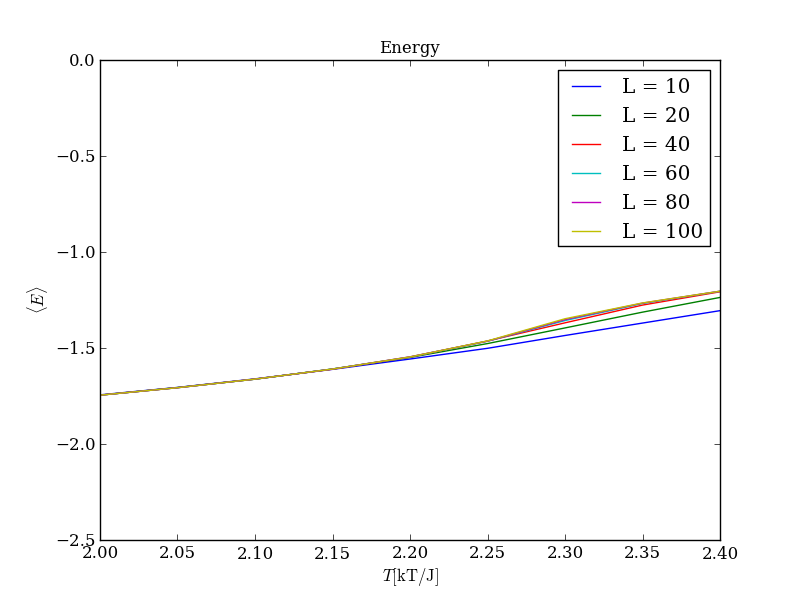
\includegraphics[width=85mm]{images/E_avg_temp.png}
	& 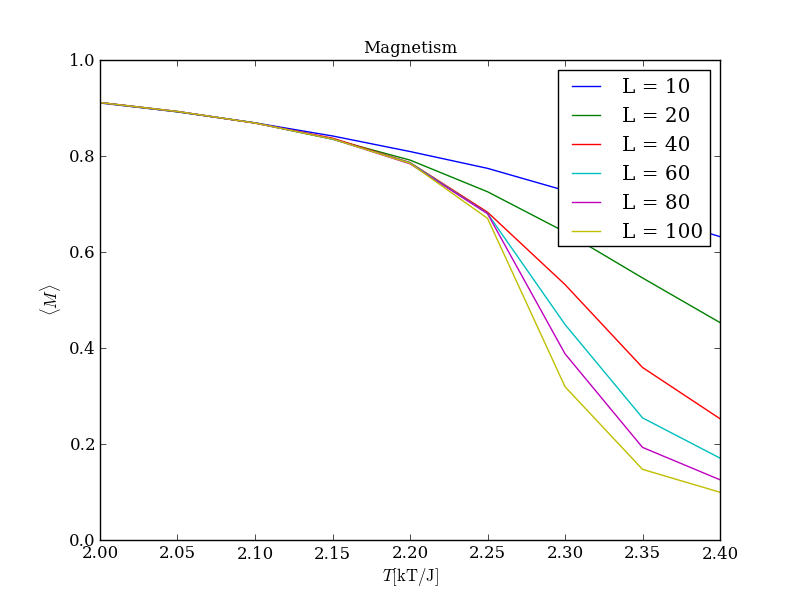
\includegraphics[width=85mm]{images/M_avg_temp.png} \\
	(a) Energy					& (b) Magnetization  \\
	
	 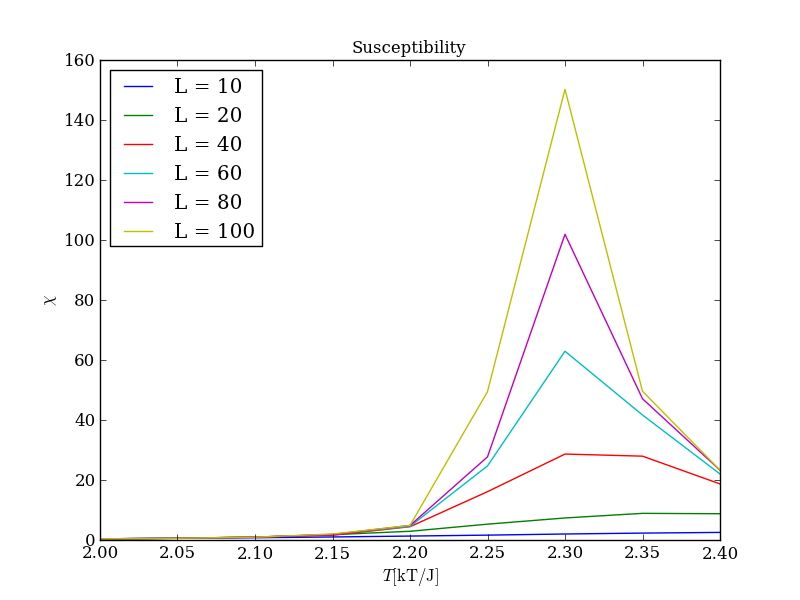
\includegraphics[width=85mm]{images/chi_temp.png}
	& 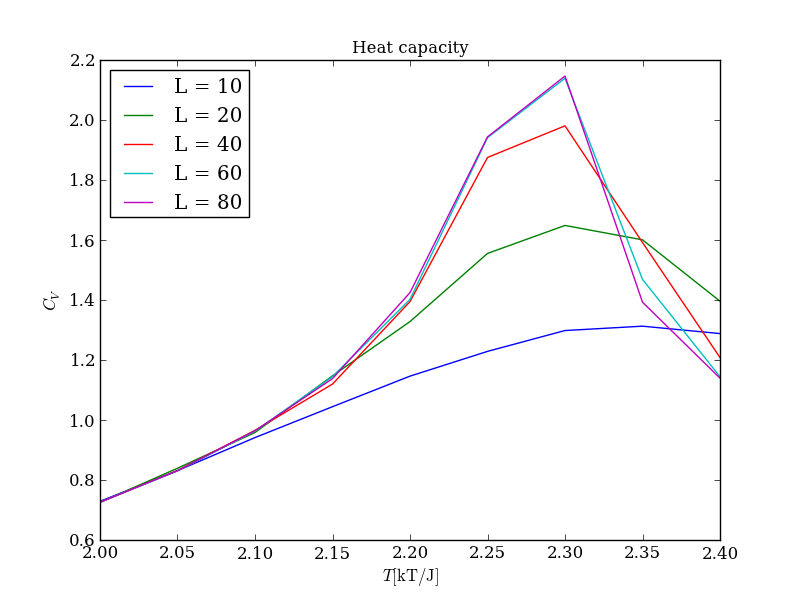
\includegraphics[width=85mm]{images/Cv_temp.png} \\
	(c) Susceptibility					& (d) Heat capacity  \\[6pt]
\end{tabular}
\caption{Expectation values as a function of temperature.}\label{fig:ex_values_temp}
\end{center}
\end{figure*}





\subsection{Estimating the critical temperature $T_{\mathrm{C}}$}

Lastly, we want to estimate the critical temperature $T_{\mathrm{C}}$ in the thermodynamic limit $L \rightarrow \infty$ using Eq. (\ref{eq:T_C}). In our study of the behaviour of our model close to the critical temperature we look at the various expectation values as a function of $T$ for $L = 20, L = 40, L = 60$ and $L = 80$ for $T \in [2.0,2.4]$, shown in Fig.~\ref{fig:ex_values_temp}a-d. Rewriting Eq. (\ref{eq:T_C}) gives

\begin{equation}\label{eg:T_C_estimate}
	T_{\mathrm{C}} = T_{\mathrm{C}}(L) - \frac{a}{L}.
\end{equation}
The calculated $T_{\mathrm{C}}(L)$ obtained from the datasets, with a temperature step length of 0.05, is listed in the following table:
\begin{center}
\begin{tabular}{ c c }
	\hline
	Lattice size $L$ & $T_C(L)$\\
	\hline
	$10$			& 2.40	\\
	$20$			& 2.35	\\
	$40$			& 2.30 	\\
	$60$			& 2.30	\\
	$80$			& 2.30	\\
	$100$			& 2.30	\\
	\hline
\end{tabular}
\end{center}
Because $T_{\mathrm{C}}(L)>T_{\mathrm{C}}$, we will never get closer to $T_{\mathrm{C}}$ no matter how large $L$ is, due to the step length. Assuming that $a$ is of the order unity, Eg. (\ref{eg:T_C_estimate}) would thus result in $T_{\mathrm{C}} = 2.3$ when $L\rightarrow\infty$.

Decreasing the temperature step length to $0.01$ could result in $T_{\mathrm{C}}(L) = 2.27$, which is a much better estimate.

% However this took far to long time, so in order to make the deadline, this was not done.

% If time: set up table with new $T_C(L)$ values, and estimate $T_C$ from them.


\subsection{Parallelization}
As described previously, we parallelized our code using MPI. Here we have gathered some time recordings, using $n = 4$ processes on a 2,5 GHz Intel Core i5 processor:

\begin{center}
\begin{tabular}{ l r }
	\hline
	Lattice size $L$ 	& Time usage $t$\\
	\hline
	$10$				& 00m 57s		\\
	$20$				& 03m 52s		\\
	$40$				& 15m 23s 		\\
	$60$				& 48m 06s		\\
	$80$				& 2h 02m 00s	\\
	$100$			& 8h 46m 22s	\\
	\hline
\end{tabular}
\end{center}
These data is plotted in Fig.~\ref{fig:time_usage}, approximated by a $L^2$ curve which makes a good fit for lower values of $L$, and a $e^{L/9.5}$ curve which is a good approximation for higher values of $L$.

\begin{center}
	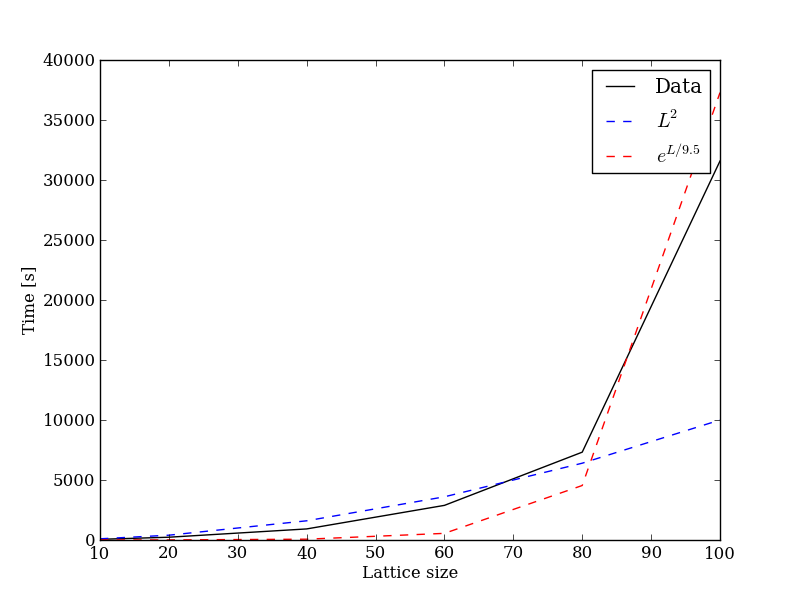
\includegraphics[width=90mm]{images/time_usage.png}	
	\captionof{figure}{Time needed to run the program as a function of lattice size.}
	\label{fig:time_usage}
\end{center}


\section{Conclusions}

We have studied the phase transition of a spin system using the Ising model in two dimensions without an external magnetic field. 

MORE.

From Fig.~\ref{fig:time_usage} it is evident that the time consumption of the code increases significantly with larger lattice size $L$, making it desirable to get away with as low a value for $L$ as possible. How low $L$ can we get away with?

Something about lattice size vs. time vs. results.

The quality of our simulation can be discussed by comparing our numerical results to the exact value of the critical temperature $T_{\mathrm{C}}$. We see that the lattice size $L$ is extremely important in some cases. Reviewing the results for the expectation values in Fig.~\ref{fig:ex_values_temp}, the value of $\langle E \rangle$ does not vary much with lattice size, but the lattice size is highly important in the case of $\langle {\cal M}\rangle$, which can tell us whether a phase transition has occurred or not. 

... MORE!







\section{List of codes}

The codes developed and used for this project are:\\

\noindent \verb@main.cpp@ -- main program (C++).

\noindent \verb@plotting.py@ -- plotting program which makes plots to study the total number of accepted configurations as a function of total number of MC cycles and as a function of temperature $T$ (Python).

\noindent \verb@visualization.py@ -- a provided program for running the Metropolis algorithm and plotting the spin matrix, as shown in Fig.~\ref{fig:visualization} (Python).

\end{multicols}

\end{document}
